\chapter{Studi Literatur}

Pada bab ini, Penulis akan menguraikan hasil studi literatur dalam penyusunan
tugas akhir ini. Subbab pertama membahas simulator CARLA, yaitu perangkat lunak
yang digunakan sebagai alat simulasi. Subbab kedua menjelaskan NVIDIA Pegasus
yang akan digunakan sebagai mesin untuk menjalankan algoritma \textit{decision
    making} di lingkungan simulasi dan \textit{production}. Lalu, pada subbab ketiga
akan dibahas beberapa cara komunikasi yang dapat digunakan pada antara server
simulator CARLA dengan NVIDIA Pegasus. Terakhir, subbab keempat akan membahas
penelitian-penelitian terkait simulasi \textit{autonomous vehicle} menggunakan
CARLA.

\section{Simulator CARLA}

CARLA (\textit{Car Learning to Act}) adalah perangkat lunak sumber terbuka
(\textit{o\-pen sour\-ce}) yang memiliki tujuan utama menyimulasikan kendaraan
autonomous. CAR\-LA dibangun dari nol untuk mampu melakukan pelatihan, pembuatan
prototipe, dan validasi model kemudi otonom, termasuk persepsi dan kontrol dari
model tersebut \parencite{dos_carla}.

\begin{figure}
    \centering
    %% TODO: Ubah ke gambar yang di-SS sendiri
    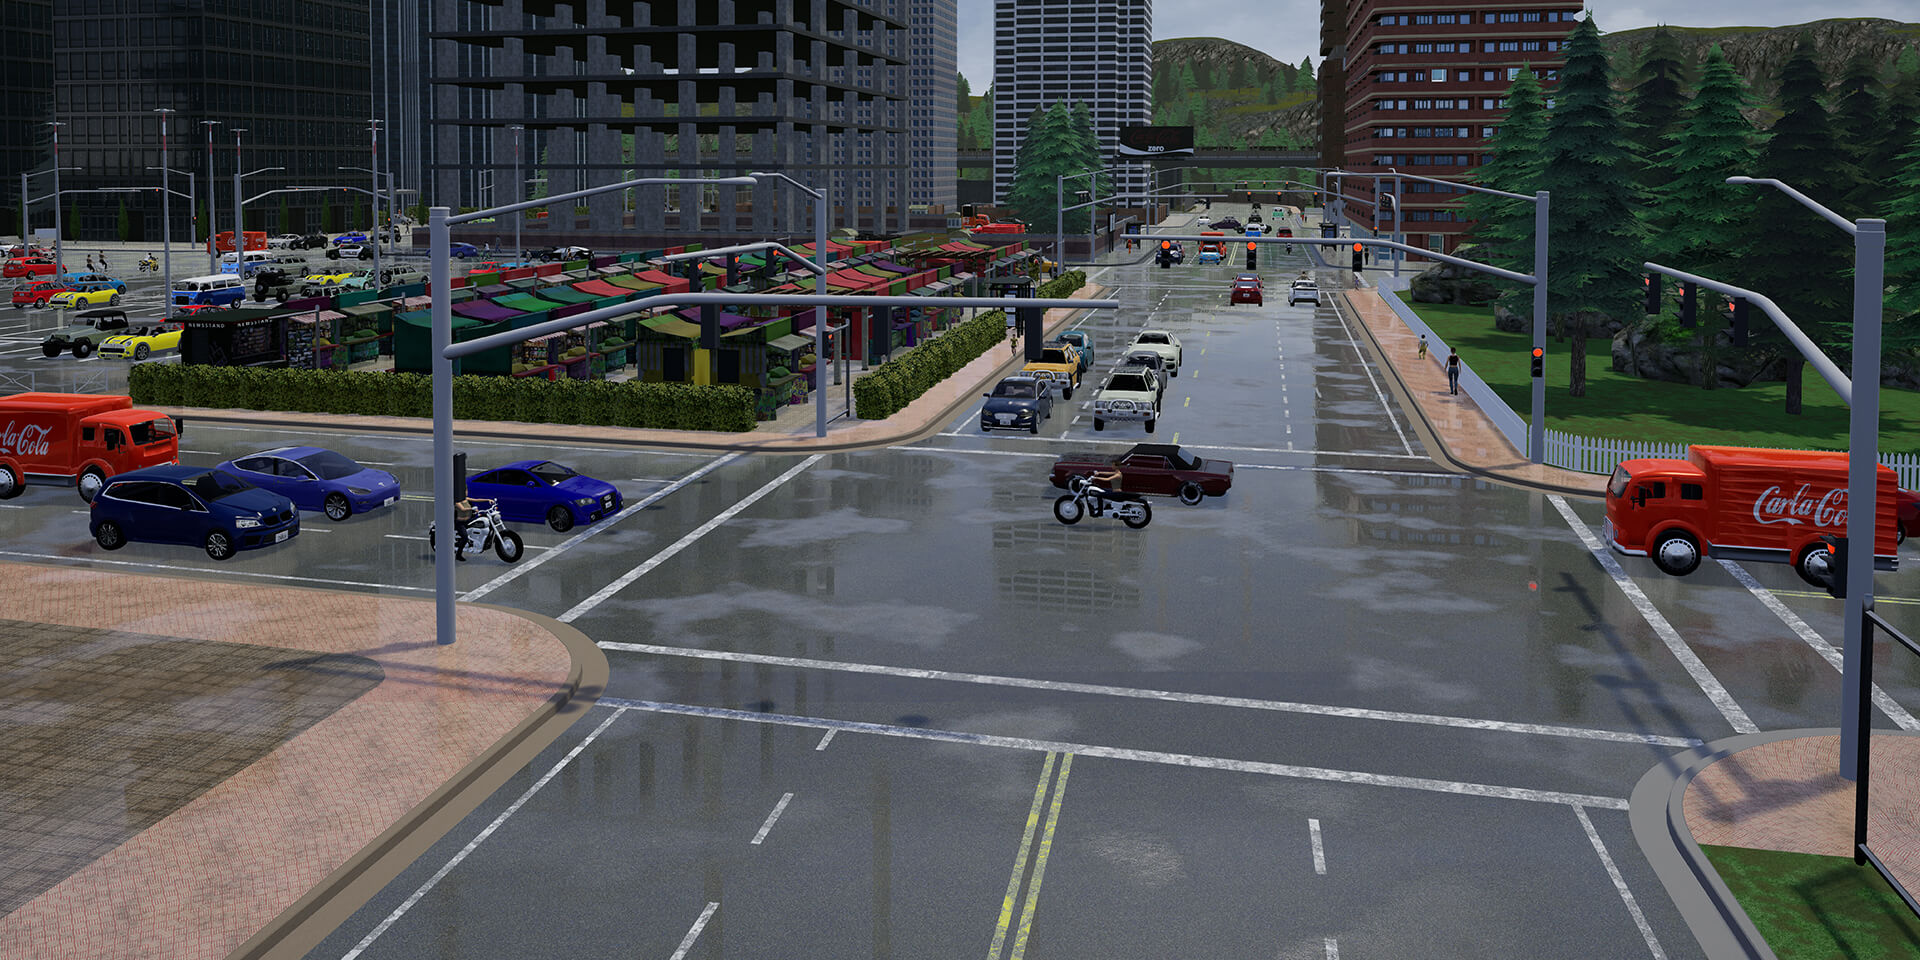
\includegraphics[width=1.0\textwidth]{resources/chapter-2/CARLA.jpg}
    \caption{Antarmuka simulator CARLA \parencite{loze_carlaDemocratizes}}
\end{figure}

CARLA sendiri dibangun di atas mesin gim (\textit{game engine}) Unreal Engine 4
(UE4). UE4 dipilih karena memiliki simulasi fisika dan kualitas grafis terbaik,
setidaknya pada saat CARLA dibuat. Selain itu, UE4 juga memiliki ekosistem untuk
pengaya (\textit{plugin}) dan sistem untuk menambahkan logika dasar untuk
(\textit{non-playable character}\footnote{Istilah untuk karakter yang tidak
    dapat dimainkan pada gim.}). UE4 dan sifat sumber terbuka CARLA memungkinkan
komunitas untuk menambahkan berbagai hal sesuai dengan kebutuhan mereka atau
bahkan memperbaiki CARLA.

Agar simulasi yang dilakukan CARLA serealistis mungkin, CARLA menyediakan
berbagai macam model 3D: kendaraan, pejalan kaki, gedung, dan rambu lalu lintas.
Model-model 3D yang disediakan dibuat dengan menggunakan teknik yang
menghasilkan bentuk dan tekstur senyata mungkin, akan tetapi tetap cepat untuk
di-\textit{render}. Model kendaraan dan pejalan kaki yang dibuat bisa memiliki
banyak variasi, misalnya kendaraan Yamaha YZF dengan warna yang berbeda atau
pejalan kaki dengan aksesoris dan pakaian yang berbeda. Model-model 3D
digunakan untuk membangun lingkungan simulasi yang realistis.

Selain dari model 3D, lingkungan simulasi yang realistis didapatkan juga dari
cuaca dan waktu hari. Cuaca dan waktu hari pada CARLA dapat dikustomisasi
se\-de\-mi\-ki\-an rupa untuk memungkinkan berbagai macam skenario simulasi.
Selain itu, NPC yang ada di CARLA akan menggunakan sebuah model dari kendaraan
ataupun pejalan kaki. NPC bergerak berdasarkan suatu aturan yang sudah
ditentukan, misalnya mengikuti suatu pemilihan keputusan ketika di lampu lalu
lintas.

Selain model, CARLA juga menyediakan berbagai sensor untuk menyimulasikan
pengambilan data. Sensor-sensor tersebut dapat ``ditempelkan'' ke kendaraan
simulasi. Contoh sensor yang tersedia adalah kamera dan LIDAR (\textit{Light
    Detection and Ranging}), dan lain-lain. Selain data dari sensor, bisa didapatkan
juga data seperti kecepatan dan percepatan (mirip dengan data dari GPS) dari
kendaraan.

CARLA bekerja dengan arsitektur server-klien. Arsitektur ini memungkinkan dunia
yang dinamis dan antarmuka yang sederhana antara dunia dan agen yang
berinteraksi dengannya. Server pada CARLA berfungsi untuk menjalankan simulasi
dan me-\textit{render scene}-nya. Lalu, klien bertugas untuk mengirimkan
perintah dan ``perintah meta'' ke server dan menerima data sensor. Perintah yang
dapat dikirimkan klien digunakan untuk mengendalikan kendaraan yang
disimulasikan. Sedangkan ``perintah meta'' digunakan untuk mengatur lingkungan
simulasi, misalnya cuaca, sensor yang digunakan, dan jumlah kendaraan/pejalan
kaki NPC.

Pada sistem simulasi TA ini, komponen klien dan server CARLA akan dijalankan
pada sebuah server simulasi. Data yang didapatkan dari CARLA akan dikirim ke
sebuah server komputasi yang menggunakan NVIDIA Pegasus.

\section{NVIDIA Pegasus}

NVIDIA Pegasus adalah salah satu produk cetusan NVIDIA Corporation di bawah lini
produk NVIDIA Drive PX. Nama pasar dari NVIDIA Pegasus adalah N\-VI\-DI\-A Drive
PX Pegasus. Lini produk NVIDIA Drive sendiri merupakan platform komputer untuk
memberikan fungsionalitas bantuan mengemudi pada kendaraan bermotor.

\begin{figure}
    \centering
    %% TODO: Foto sendiri (?)
    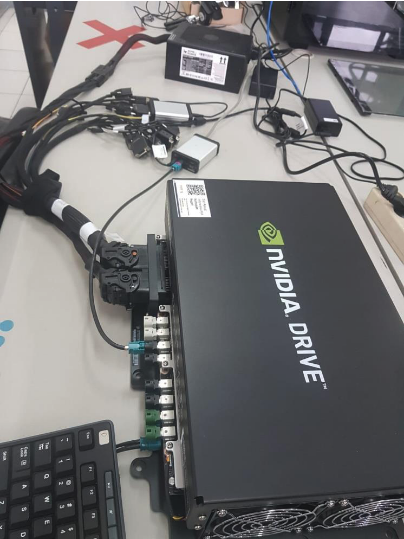
\includegraphics[width=\textwidth]{resources/chapter-2/pegasus.png}
    \caption{NVIDIA Pegasus \parencite{trilaksono_laporanRispro}}
\end{figure}

Mengutip dari \parencite{oh_2017}, NVIDIA Pegasus adalah komputer yang mendukung
pengemudian \textit{autonomous} secara penuh. Artinya, NVIDIA Pegasus dapat
digunakan untuk membuat sebuah kendaraan bermotor menjadi \textit{autonomous
    vehcile} jika sensor dan algoritma yang digunakan tepat.

NVIDIA Pegasus menggunakan 2 GPU dengan arsitektur post-Volta dan 2 SoC NVIDIA
Xavier. Kombinasi CPU dan GPU ini dapat menghasilkan 320 TOPS (\textit{trillion
    operations/second}) untuk komputasi intelegensi buatan. Untuk koneksi I/O,
NVIDIA Pegasus mendukung sampai dengan 16 kamera (6 di antaranya adalah lidar).

Pada sistem simulasi yang dibuat, NVDIA Pegasus akan menjadi server yang
ber\-tang\-gung jawab atas komputasi serta \textit{decision making}. NVIDIA
Pegasus yang digunakan memiliki kumpulan kakas dan pustaka untuk membangun
aplikasi robot yang disebut ROS (\textit{robot operating system}) sehingga dapat
menjadi \textit{node} ROS.

\section{Metode Komunikasi antara Simulator CARLA dan NVI\-DI\-A Pegasus}

Pada keadaan yang ada, komunikasi antara simulator CARLA dengan NVIDIA Pegasus
menggunakan perantara \textit{web service} yang berbasis HTTP/1.1. Penggunaan
HTTP/1.1 pada \textit{web service} menjadi \textit{bottleneck}/penghambat
kinerja terbesar sistem simulasi. Ketika dilakukan secara SILS (\textit{software
    in the loop simulation} tanpa NVIDIA Pegasus) didapatkan kinerja 4000 transaksi
per detik, sedangkan ketika NVIDIA Pegasus ditambahkan ke sistem (menjadi HILS,
\textit{hardware in the loop simulation}) didapatkan 100--110 transaksi per
detik \parencite{trilaksono_laporanRispro}. Oleh karena itu, dibutuhkan protokol
atau metode komunikasi lain yang dapat meningkatkan kinerja jalur komunikasi.
Selain itu, jalur komunikasi yang digunakan harus dapat mengirimkan pesan berupa
teks \textit{string}, larik angka, atau data \textit{binary} (misalnya gambar).

\begin{figure}
    \centering
    \includegraphics[width=1.0\textwidth]{resources/chapter-2/komunikasi
        data pada simulasi.png}
    \caption{Arsitektur komunikasi pada HILS
        \parencite{trilaksono_laporanRispro}}
\end{figure}

Beberapa alternatif metode jalur komunikasi dapat digunakan untuk
meng\-hu\-bung\-kan kedua server akan dibahas pada subbab ini. metode tersebut
adalah komunikasi berorientasi pesan dan RPC.

\subsection{RPC}

RPC, atau \textit{remote procedure call}, secara teknis bukanlah protokol,
melainkan sebuah mekanisme untuk menyusun sistem terdistribusi yang
berkomunikasi dengan pola \textit{request/reply}
\parencite{larry_computerNetwork}. RPC memberikan abstraksi kepada pengembang
berupa pemanggilan fungsi secara lokal maupun \textit{remote}, di permukaannya,
memiliki perilaku yang sama. Pemanggilan fungsi \textit{remote} artinya
implementasi fungsi berada di komputer lain di dalam jaringan.

Ketika menggunakan RPC, pengembang tidak perlu tahu pemanggilan sebuah fung\-si
dilakukan secara lokal atau \textit{remote}; pengembang hanya perlu tahu
pemanggilan fungsi tersebut akan menghasilkan suatu nilai baru dan berpotensi
membuat program \textit{blocking} (menunggu) sampai nilai baru tersebut
didapatkan\footnote{terdapat variasi RPC, \textit{asynchronous} RPC, yang
    memungkinkan pemanggilan fungsi \textit{remote} tanpa menghasilkan
    \textit{return} sehingga tidak perlu ditunggu.}.

Implementasi RPC yang akan dibahas pada subbab ini adalah gRPC. gRPC juga
merupakan implementasi RPC yang akan digunakan untuk membangun jalur komunikasi
antara server NVIDIA Pegasus dengan server simulator CARLA. gRPC dipilih karena
kemampuannya mengirimkan pesan dalam format \textit{binary} dan mengirimkan
pesan secara \textit{streaming}. Akan tetapi, gRPC bukan merupakan implementasi
RPC dengan kinerja dan efisiensi penggunaan \textit{resource} komputer terbaik
\parencite{chris_rpc_benchmark}. Kendati demikian, fitur \textit{streaming} data
dinilai lebih penting daripada efisiensi \textit{resource} pada \textit{use
    case} simulasi ini.

\subsubsection{gRPC}

gRPC adalah salah satu implementasi RPC dalam bentuk \textit{framework} dari
Google. Google merilis gRPC proyek sumber terbuka pada tahun 2016. Teknologi
gRPC datang dari teknologi internal di Google bernama Stubby. Google merilis
Stubby menjadi gRPC ke publik untuk menstandardisasi Stubby dengan standard
baru: HTTP/2, SPDY, dan QUIC. Selain itu, untuk memperluas fungsionalitas Stubby
agar dapat digunakan untuk aplikasi \textit{mobile}, IoT, dan komputasi awan
\parencite{ryan_grpcPricinples}.

gRPC dapat digunakan di berbagai bahasa pemrograman. Secara bawaan, gRPC
mendukung 10 bahasa. Untuk mendukung banyak bahasa dan memberikan abstraksi,
gRPC memiliki tiga jenis arsitektur. Arsitektur-arsitektur tersebut adalah
arsitektur untuk ``bahasa terbungkus'' (\textit{wrapped languages}), Go, dan
Java. Tugas akhir ini akan menggunakan bahasa Python dan C++ sehingga hanya
arsitektur untuk ``bahasa terbungkus'' yang dijelaskan secara detail. Arsitektur
gRPC untuk ``bahasa terbungkus'' dapat dilihat pada gambar
\ref{chapter-2-grpc-stack}.

\begin{figure}
    \centering
    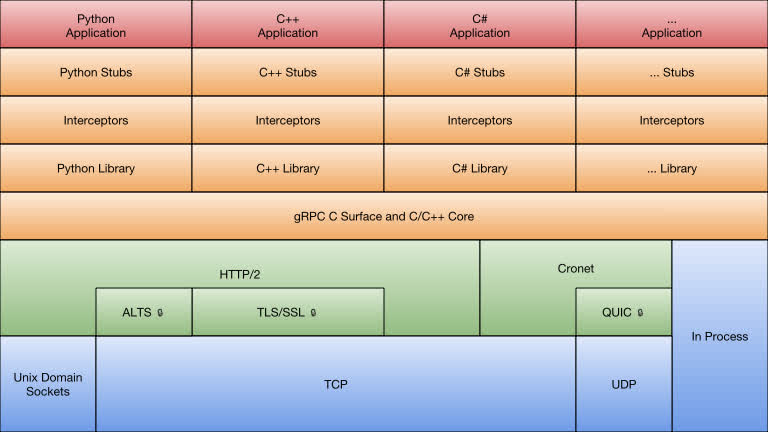
\includegraphics[width=1.0\textwidth]{resources/chapter-2/grpc-arch.jpeg}
    \caption{Arsitektur gRPC untuk ``bahasa terbungkus''
        \parencite{mastrangelo_grpcStack}}
    \label{chapter-2-grpc-stack}
\end{figure}

Pada ``bahasa terbungkus'', pemanggilan prosedur \textit{remote} menggunakan
gRPC me\-la\-lu\-i sebuah \textit{stub} yang me\-le\-wa\-ti
\textit{interceptor}. Lalu, pemanggilan dari \textit{stub} akan dilanjutkan ke
pustaka pembungkus (\textit{wrapper}) untuk tiap bahasa yang
me\-ner\-je\-mah\-kan pemanggilan tadi ke pemanggilan fungsi C. Fungsi C yang
dipanggil adalah bagian dari C-core. C-core pustaka gRPC untuk mengabstraksikan
lapisan transpor. Secara bawaan, C-core akan menggunakan HTTP/2 sebagai
lapisan transpor \parencite{mastrangelo_grpcStack}.

\textit{Stub} pada arsitektur gRPC dibangkitkan (\textit{generate}) dari IDL
(\textit{interface definion language}). gRPC dapat menggunakan IDL yang
berbeda-beda, tapi yang memberikan dukungan terhadap gRPC baru Protocol Buffer
(protobuf) dan Flatbuffers. Pengguna gRPC harus mendefinisikan layanan
(\textit{service}), struktur data, dan \textit{enum} yang dapat digunakan pada
IDL. Layanan yang diberikan kemudian diimplementasikan di sisi server.

Ketika melakukan RPC, gRPC akan menserialisasi data menjadi format tertentu yang
dikirim melaui lapisan transpor, misalnya HTTP/2. Penerima (server) akan
mendeserialisasi data tersebut lalu menjalankan prosedur/fungsi terkait. Setelah
itu, \textit{return} dari fungsi/prosedur akan diserialisasi dan dikembalikan ke
pengirim. Format serialisasi tergantung pada metode serialisasi yang digunakan
dan berkaitan erat dengan IDL yang digunakan. Pada tugas akhir ini, IDL dan metode
serialisasi yang akan digunakan adalah protobuf, artinya data akan
diserialisasikan menjadi larik dari \textit{byte}.

\subsection{Komunikasi Berorientasi Pesan}

Komunikasi berorientasi pesan adalah salah satu metode komunikasi pada sistem
terdistribusi. Metode ini utamanya bersifat
\textit{asynchronous}\footnote{Beberapa implementasi bisa \textit{synchronous}
    juga.}, artinya konsumen/klien tidak perlu \textit{blocking} ketika membuat
\textit{request}. Sifat \textit{asynchronous} ini merupakan alternatif untuk
serta cara berkomunikasi \textit{request/response} lainnya dan berguna ketika
konsumen tidak membutuhkan hasil pemrosesan pesan.

Selain sifat \textit{asynchronous}, keunggulan lain dari komunikasi berorientasi
pesan ada\-lah menghilangkan kebutuhan mesin ``server'' (yang mengeksekusi) pesan
tidak harus sedang berjalan ketika pesan dikirimkan. Tidak seperti RPC yang
mengharuskan mesin server dan klien berjalan agar pemanggilan fungsi
\textit{remote} dapat berjalan.

Implementasi untuk komunikasi berorientasi pesan yang akan dibahas adalah ROS
dan pustaka ZeroMQ. Kedua protokol juga akan digunakan untuk membuat jalur
komunikasi antara server NVIDIA Pegasus dengan server simulator CARLA.

% TODO: apa iya masih message-oriented?
\subsubsection{ROS 2}

ROS 2 adalah peningkatan dari ROS. ROS adalah kependekan dari \textit{robot
    operating system} dan merupakan sekumpulan pustaka dan kakas perangkat lunak
untuk membangun aplikasi robotik. ROS 2 dibuat karena ROS menunjukkan masalah di
sektor keamanan, reliabilitas, dan penggunaan pada aplikasi skala besar
\parencite{doi:10.1126/scirobotics.abm6074_ros}. Misalnya, ROS memiliki satu
titik kegagalan, sedangkan masalah ini tidak ada di ROS 2.

ROS dilengkapi dengan berbagai macam kakas dan perangkat lunak, mulai dari
\textit{driver} sampai kakas pemrograman. ROS dapat menyediakan fitur serupa
dengan sistem operasi, misalnya abstraksi perangkat keras, kendali perangkat
\textit{low-level}, implementasi fungsionalitas yang sering digunakan,
\textit{message-passing} antar-proses, dan \textit{package management}
\parencite{x_rosIntro}.  Meskipun demikian ROS bukan sistem operasi ``nyata''
seperti Linux, Windows, ataupun MacOS karena ROS harus diinstal di atas sistem
operasi ``nyata'' tersebut.

Setiap perangkat lunak pada ROS diorganisir menjadi \textit{packages}. Setiap
\textit{package} dapat mengandung proses (\textit{node}), himpunan data,
pustaka, dan lain-lain. \textit{Package} adalah struktur terkecil dari sebuah
artifak pada ROS. Sebuah \textit{package} yang mengandung proses dapat
di-\textit{run} untuk menjalankan sebuah proses komputasi.

Proses-proses yang melakukan komputasi pada ROS disebut \textit{node} di level
graf komputasi. Disebut graf karena setiap \textit{node} di ROS saling terhubung
satu sama lain membentuk sebuah jaringan \textit{peer-to-peer}. Sebuah
\textit{node} dibuat agar skalanya \textit{fine-grained} dan bertanggung jawab
hanya pada satu hal. Dalam kasus ini, ROS mirip dengan \textit{service}/layanan
pada arsitektur \textit{microservice}.

Antar-\textit{node} ROS dapat berkomunikasi dengan tiga metode, yaitu
\begin{itemize}
    \item \textit{topic}: komunikasi asinkron dengan pola
          \textit{publisher}-\textit{subscriber},
    \item \textit{service}: komunikasi secara asinkron dengan pola
          \textit{request}-respon seperti RPC, dan
    \item \textit{action}: mendeskripsikan sebuah aksi.
\end{itemize}
Pada tugas akhir ini, hanya akan digunakan \textit{topic} dan \textit{service}.
Setiap \textit{topic} dapat memiliki sebuah berkas \texttt{.msg} yang
menjelaskan isi pesan \textit{topic} apabila tidak menggunakan tipe data
sederhana (\textit{string}, \textit{integer}, dll.). Selain itu, setiap
\textit{service} juga harus didefinsikan melalui sebuah berkas IDL \texttt{.srv}
yang menjelaskan bentuk \textit{request} dan respon.

ROS2 didasarkan pada DDS untuk komunikasinya. DDS secara bawaan mendukung
komunikasi dengan pola \textit{publisher}-\textit{subscriber} dengan QoS
(\textit{quality of service}). Komunikasi dengan \textit{topic} memanfaatkan
pola tersebut. Lalu, untuk pola \textit{service}, digunakan perpanjangan dari
DDS, yaitu DDS-RPC. DDS sendiri sebenarnya hanya standar dengan implementasi
yang berbeda-beda. Secara bawaan, ROS 2 menggunakan Fast DDS dari eProsima.

Pemanfaatan DDS ini diabstraksikan oleh ROS menggunakan beberapa pustaka untuk
memudahkan pengembangan aplikasi ROS. Aplkasi yang ditulis akan memanfaatkan
API pustaka klien, misalnya \texttt{rclpy} (untuk Python). API pustaka klien
melakukan pemanggilan ke antarmuka pustaka klien yang disebut \texttt{rcl}.
\texttt{rcl} memberikan akses ke graf ROS dan kejadian (\textit{events}) pada
graf. \texttt{rcl} juga mengatur siklus hidup \textit{node} di antara beberapa
hal lainnya. \texttt{rcl} akan memanfaatkan \texttt{rmw} (antarmuka
\textit{middleware} ROS). \texttt{rmw} memberikan abstraksi dari
\textit{middleware} (atau lapisan transpor) yang digunakan.

\subsubsection{ZeroMQ}

ZeroMQ (\textit{zero message queue}) adalah sebuah pustaka yang merupakan
pe\-ning\-ka\-tan di atas \textit{socket} tradisional. ZeroMQ memberikan
fungsionalitas tambahan terhadap \textit{socket} dan mengabstraksi pembuatan
koneksi TCP dengan harapan memudahkan pengembangan aplikasi terdistribusi.
Fungsionalitas yang ditambahkan oleh ZeroMQ didasarkan pada pola-pola komunikasi
yang sering terjadi ketika menggunakan protokol TCP.

ZeroMQ memungkinkan komunikasi \textit{one-to-one} (seperti \textit{socket}
biasa), \textit{many-to-one} (\textit{socket} mendengarkan ke beberapa
\textit{port}), dan \textit{one-to-many}. Pola komunikasi yang didukung oleh
ZeroMQ adalah \textit{request-reply}, \textit{publish-subscribe}, dan
\textit{pipeline}. ZeroMQ juga memiliki sebuah antrian pesan (\textit{message
    queue}) sehingga pesan yang dikirimkan ke konsumen akan disimpan
sampai konsumen siap menerima pesan. Meskipun terhadap antrian pesan, ZeroMQ
tidak memiliki \textit{message broker}\footnote{\textit{zero} pada ZeroMQ
    artinya nol \textit{broker}, nol latensi, nol biaya, dan nol administrasi.}.

ZeroMQ berjalan di atas lapisan transpor ZMTP (ZeroMQ \textit{message transport
    protocol}). Semantik ZMTP memastikan pesan tidak akan diterima lebih dari 1 kali
oleh konsumen dan semua pesan akan diterima oleh konsumen dengan urutan yang
benar. Selain itu, \textit{frame} pesan yang diterima konsumen akan
di-\textit{queue} di memori penerima sampai semua \textit{frame} diterima.
Semantik ZMTP juga memastikan \textit{socket} dapat membuat dan menerima koneksi
serta \textit{socket} akan menyambungkan kembali jika koneksi terputus.

\section{Penelitian Terkait}

Terdapat sebuah penelitian yang memiliki lingkup serta lingkungan sama dengan
tugas akhir ini. Penelitian tersebut juga menggunakan CARLA untuk HILS.

\subsection{\textit{Hardware-in-the-Loop Autonomous Driving Simulation Without
        Real-Time Constraints}}

Pada penelitian ini \parencite{brogle_CarlaHILS}, dilakukan HILS menggunakan
NVIDIA Jetson TX1 sebagai perangkat keras untuk komputasi dan simulasi
menggunakan simulator CARLA. Salah satu hasil dari penelitian ini adalah
integrasi antara simulator CARLA dengan kakas ROS.

Arsitektur untuk menggunakan ROS dalam simulasi HILS dapat dilihat pada gambar
\ref{chapter-2-carla-jetson-arch}. Terdapat sebuah \textit{node}  yang
bertugas mendapatkan data kamera dan LiDAR dari CARLA. Kemudian, data tersebut
dipublikasikan ke topik yang didengarkan oleh pemroses data LiDAR dan vidio.
\textit{Node} yang terhubung dengan CARLA akan dikirimkan data terkait kendali
kendaraan oleh \textit{node} yang disebut \textit{path planning node}.

\begin{figure}
    \centering
    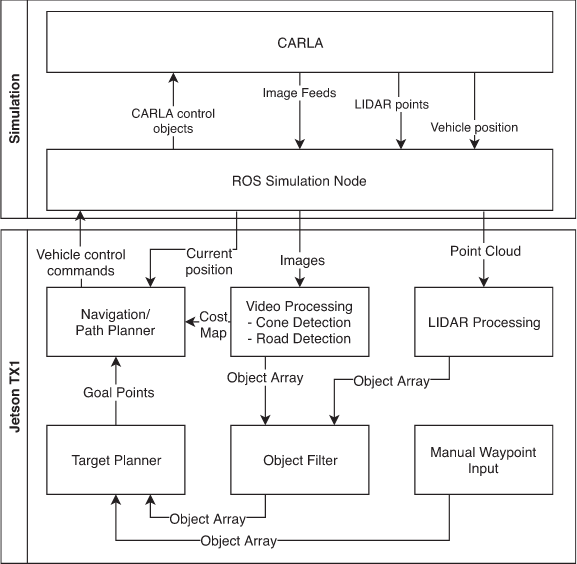
\includegraphics[width=1.0\textwidth]{resources/chapter-2/carla-jetson-arch.png}
    \caption{Arsitektur sistem simulasi \parencite{brogle_CarlaHILS}}
    \label{chapter-2-carla-jetson-arch}
\end{figure}

Hasil eksperimen pada penelitian ini adalah hasil simulasi menggunakan HILS dan
CARLA tidak berbeda jauh dengan keadaan dunia nyata. Selain itu, didapatkan juga
waktu respons pada sistem simulasi lebih cepat dari dunia nyata. Sehingga, dapat
disimpulkan bahwa simulasi HILS dapat dilakukan dan implementasi dengan
menggunakan ROS (tanpa rosbridge) sudah memberikan hasil yang baik.
